\section{Architettura}

%%%%%%%%%%%%%%%%%%%%%%%%%%%%%%%%%%%%%%%%%%%%%%%%%%%%%%%%%%%%%%%%%%%%%%%%%%%%%%%%%%
\subsection{Introduzione all’architettura}
    \subsubsection{Scopo e obbiettivi}
    La presente sezione ha lo scopo di fornire una visione d’insieme dell’architettura del sistema, evidenziandone i principi guida e le scelte progettuali che ne hanno determinato la struttura. In particolare, si intende:
    \begin{itemize}
        \item Definire il contesto in cui opera il sistema, evidenziando i requisiti funzionali e non funzionali che hanno condotto alla scelta di una specifica architettura.
        \item Orientare i lettori (sviluppatori, progettisti e stakeholder) verso una comprensione chiara delle componenti principali e delle interazioni che caratterizzano il sistema.
        \item Porre le basi per la discussione delle scelte di design, evidenziando come queste possano rispondere alle esigenze di scalabilità, sicurezza, manutenibilità e performance.
        \item Descrivere le motivazioni alla base delle scelte tecnologiche e dei modelli architetturali adottati.
    \end{itemize}



%%%%%%%%%%%%%%%%%%%%%%%%%%%%%%%%%%%%%%%%%%%%%%%%%%%%%%%%%%%%%%%%%%%%%%%%%%%%%%%%%%

\subsection{Architettura del sistema}
La progettazione dell’architettura del sistema ha richiesto un’approfondita analisi delle due principali opzioni architetturali disponibili: \textbf{monolitica} e \textbf{a microservizi}. La scelta dell’architettura è stata guidata da una serie di fattori, tra cui la natura dell’applicazione, il volume di traffico previsto, i costi di sviluppo e manutenzione e la necessità di scalabilità. In questa sezione verranno analizzati nel dettaglio i pro e i contro di entrambe le soluzioni, per poi motivare la decisione finale.
\subsubsection{Architettura monolitica}
Un’architettura monolitica si basa su un’unica codebase che incorpora tutti i componenti dell’applicazione, tra cui l’interfaccia utente, la logica di business e il livello di accesso ai dati. Questo approccio, tradizionalmente adottato nello sviluppo software, è particolarmente indicato per applicazioni di piccola e media complessità, in cui i costi di separazione dei componenti in unità indipendenti non sono giustificati.
\paragraph{Vantaggi}  
\begin{itemize}
    \item \textbf{Semplicità di sviluppo e gestione}: Un’unica codebase permette di mantenere una visione centralizzata del sistema, semplificando lo sviluppo, il testing e il debugging.
    \item \textbf{Minori costi di infrastruttura}: Non è necessario investire in strumenti di orchestrazione, load balancing o gestione della comunicazione tra microservizi.
    \item \textbf{Deployment più semplice}: L’intero sistema viene distribuito come un’unica unità, evitando problemi di coordinamento.
    \item \textbf{Prestazioni migliori per bassi volumi di traffico}: L’assenza di chiamate di rete tra microservizi riduce la latenza.
\end{itemize}
\paragraph{Svantaggi}  
\begin{itemize}
    \item \textbf{Scalabilità limitata}: Non è possibile scalare singole componenti separatamente.
    \item \textbf{Maggiore impatto degli errori}: Un bug in una parte dell’applicazione può compromettere l’intero sistema.
    \item \textbf{Difficoltà nell’adozione di nuove tecnologie}: L’aggiornamento di singole parti è complesso poiché l’intero stack è integrato.
\end{itemize}

\subsubsection{Architettura a microservizi}
L’architettura a microservizi suddivide il sistema in componenti indipendenti, ognuno responsabile di una funzionalità specifica. Ogni microservizio comunica con gli altri attraverso API, permettendo un alto grado di indipendenza e flessibilità nello sviluppo.
\paragraph{Vantaggi}  
\begin{itemize}
    \item \textbf{Scalabilità orizzontale}: Ogni microservizio può essere scalato indipendentemente.
    \item \textbf{Flessibilità nello sviluppo}: Permette l’adozione di tecnologie diverse per ciascun servizio.
    \item \textbf{Maggiore resilienza}: Un errore in un microservizio non compromette l’intero sistema.
    \item \textbf{Facilità di manutenzione}: È possibile distribuire aggiornamenti senza dover ripubblicare l’intera applicazione.
\end{itemize}
\paragraph{Svantaggi}  
\begin{itemize}
    \item \textbf{Maggiore complessità gestionale}: L’orchestrazione dei microservizi richiede strumenti avanzati.
    \item \textbf{Comunicazione tra servizi}: Introduce latenza e potenziali colli di bottiglia.
    \item \textbf{Deployment più complesso}: Coordinare il rilascio di più servizi è più oneroso.
    \item \textbf{Costi di sviluppo più elevati}: La frammentazione del sistema richiede maggiore sforzo di progettazione e testing.
\end{itemize}

\subsubsection{Scelta del monolite esagonale}
Dopo un’analisi approfondita, il team di sviluppo ha deciso di adottare un’\textbf{architettura monolitica esagonale}. Questa scelta è stata motivata dai seguenti fattori:
\begin{enumerate}
    \item \textbf{Basso carico di utenti}: L’applicazione è destinata a un contesto B2B con un numero limitato di utenti concorrenti.
    \item \textbf{Semplicità di gestione}: La manutenzione di un monolite è più diretta rispetto a un sistema distribuito.
    \item \textbf{Riduzione dei costi operativi}: L’assenza di strumenti di orchestrazione riduce significativamente i costi di infrastruttura.
    \item \textbf{Velocità di sviluppo}: Un’unica codebase consente iterazioni rapide senza dipendenze tra servizi separati.
    \item \textbf{Evoluzione graduale verso microservizi}: Adottando un’architettura \textbf{esagonale}, il sistema può essere trasformato gradualmente in microservizi senza riscrivere tutto.
\end{enumerate}

\subsection{Architettura esagonale}
L’\textbf{architettura esagonale}, nota anche come \textit{Ports and Adapters}, è un pattern architetturale l'obiettivo di rendere il software più flessibile, testabile e indipendente dalle tecnologie esterne. Questo approccio enfatizza la separazione tra la logica di business e le interfacce di comunicazione con il mondo esterno.

\subsubsection{Principi fondamentali}
L'architettura esagonale si basa su tre concetti chiave:
\begin{itemize}
    \item \textbf{Isolamento della logica di business}: Il core dell'applicazione è indipendente dai dettagli implementativi esterni.
    \item \textbf{Utilizzo di porte e adattatori}: Le \textit{porte} definiscono le interfacce per la comunicazione tra il core e il mondo esterno, mentre gli \textit{adattatori} implementano queste interfacce per specifiche tecnologie.
    \item \textbf{Sostituibilità delle dipendenze}: È possibile cambiare database, framework web o altre dipendenze senza impattare il core.
\end{itemize}

\subsubsection{Struttura dell’architettura esagonale}
L’architettura esagonale può essere rappresentata con tre livelli principali:
\begin{enumerate}
    \item \textbf{Core (Dominio e Logica di Business)}: Contiene le regole fondamentali dell’applicazione.
    \item \textbf{Porte (Ports)}: Interfacce che definiscono i punti di ingresso e uscita del sistema.
    \item \textbf{Adattatori (Adapters)}: Implementazioni concrete delle porte per database, servizi esterni e UI.
\end{enumerate}
\begin{figure}[H]
    \centering
    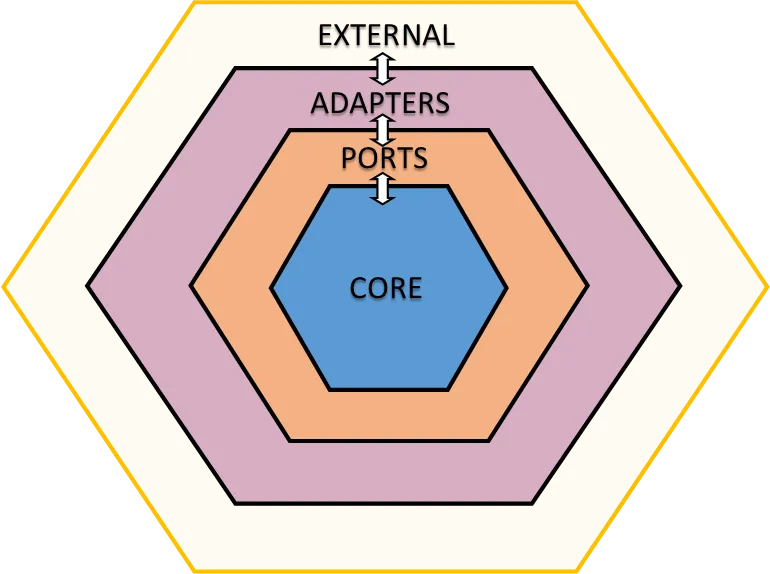
\includegraphics[width=0.7\textwidth]{./img/hexagonal_architecture.png}
    \caption{Schema dell'architettura esagonale}
    \label{fig:hex_arch}
\end{figure}

\subsubsection{Vantaggi dell’architettura esagonale}
Adottare un'architettura esagonale comporta diversi benefici:
\begin{itemize}
    \item \textbf{Maggiore manutenibilità}: Il codice è modulare e separato.
    \item \textbf{Facilità di test}: Il core dell’applicazione può essere testato isolatamente.
    \item \textbf{Indipendenza dalle tecnologie}: Cambiare framework o database ha un impatto minimo.
    \item \textbf{Flessibilità evolutiva}: Permette di trasformare gradualmente il monolite in microservizi.
\end{itemize}

\subsubsection{Conclusione}
L’architettura esagonale garantisce modularità e sostenibilità del sistema nel lungo termine, permettendo di scalare senza impattare la stabilità complessiva dell’applicazione.







%%%%%%%%%%%%%%%%%%%%%%%%%%%%%%%%%%%%%%%%%%%%%%%%%%%%%%%%%%%%%%%%%%%%%%%%%%%%%%%%%%
\subsection{Moduli}
\subsubsection{Architettura Esagonale}
\begin{figure}[H]
    \centering
    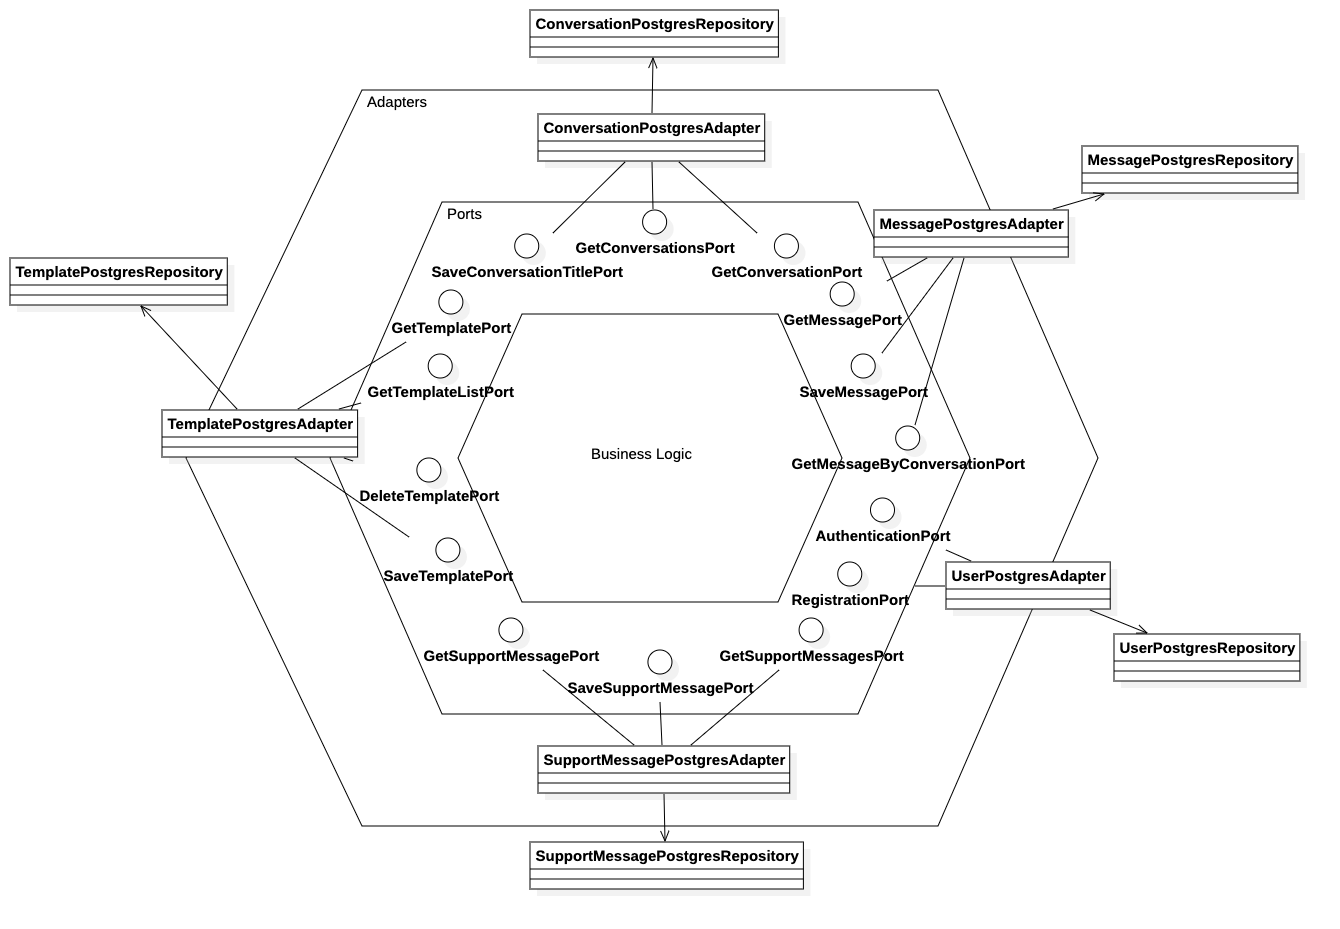
\includegraphics[width=\linewidth, height=0.8\textheight, keepaspectratio]{./img/ArchitetturaEsagonaleStarUML.png}
    \caption{Diagramma delle classi - Architettura Esagonale}
    \label{fig:architettura_esagonale}
\end{figure}




\subsubsection{Chat Controller}
\paragraph{1. Data Transfer Objects (DTO)}
\begin{itemize}
    \item \textbf{AnswerDTO \& QuestionDTO:}
    \begin{itemize}
        \item Questi oggetti sono usati per trasferire i dati tra le varie componenti (ad esempio, tra il controller e il caso d’uso).
        \item AnswerDTO incapsula la risposta generata.
        \item QuestionDTO contiene informazioni relative all’utente (identificato da un intero) e alla domanda posta.
    \end{itemize}
\end{itemize}

\paragraph{2. Modelli ed Entità}
\begin{itemize}
    \item \textbf{Modelli (Models):}
    \begin{itemize}
        \item Rappresentano le strutture dati a livello di dominio, per esempio:
        \begin{itemize}
            \item \textit{QuestionModel}: Tiene traccia dell’ID utente e del testo della domanda.
            \item \textit{AnswerModel}: Incapsula la risposta generata.
            \item \textit{ContextModel}: Utilizzato per rappresentare il contesto (ad esempio, contenuti estratti da documenti) che verrà usato per generare una risposta.
        \end{itemize}
    \end{itemize}
    \item \textbf{Entità:}
    \begin{itemize}
        \item Gli oggetti di tipo entità, come DocumentContextEntity, QueryEntity e AnswerEntity, rappresentano versioni “di basso livello” degli stessi concetti, ma con logiche e metodi per accedere ai dati (ad esempio, \texttt{get\_content()} o \texttt{get\_query()}).
        \item Queste entità sono utili per trasformare i dati dai modelli alle strutture usate nelle operazioni di business.
    \end{itemize}
\end{itemize}

\paragraph{3. Repositories e Interazione con il Vector Store}
\begin{itemize}
    \item \textbf{FaissRepository:}
    \begin{itemize}
        \item Questo componente interagisce direttamente con un vector store basato su FAISS.
        \item \texttt{similarity\_search(query)}: Riceve una QueryEntity, esegue una ricerca di similarità sul vector store (limitata ad un certo numero di risultati, ad esempio 4) e trasforma i documenti trovati in oggetti DocumentContextEntity.
        \item \texttt{load\_chunks(chunks)}: Consente di caricare “chunk” di testo (rappresentati come FileChunkEntity) nel vector store. Per ciascun chunk viene creato un oggetto Document con metadati, successivamente il vector store viene salvato in maniera persistente.
    \end{itemize}
\end{itemize}

\paragraph{4. Integrazione con LangChain}
\begin{itemize}
    \item \textbf{LangChainRepository:}
    \begin{itemize}
        \item Utilizza le funzionalità di LangChain per la generazione di risposte e per la suddivisione dei file.
        \item \texttt{generate\_answer(query, contexts, prompt\_template)}:
        \begin{enumerate}
            \item Prepara una lista di documenti (tramite Document di LangChain) a partire dai contesti ricevuti.
            \item Recupera la “memoria” utente per mantenere la storia delle conversazioni, la quali vengono trimmate se troppo lunghe per non superare un limite di token.
            \item Costruisce dinamicamente un prompt (usando ChatPromptTemplate) che include istruzioni di sistema, la storia della conversazione, la domanda attuale e il contesto.
            \item Invoca una catena (chain) per ottenere la risposta dall’LLM.
            \item Salva l’interazione nella memoria utente e restituisce la risposta incapsulata in un AnswerEntity.
        \end{enumerate}
        \item \texttt{split\_file(file)}: Suddivide il contenuto di un file in “chunk” di dimensioni definite (ad es. 2500 caratteri) utilizzando lo RecursiveCharacterTextSplitter. Se il contenuto è in bytes, viene decodificato in stringa. Il risultato è una lista di oggetti FileChunkEntity.
    \end{itemize}
\end{itemize}

\paragraph{5. Adattatori (Adapters)}
\begin{itemize}
    \item \textbf{FaissAdapter:}
    \begin{itemize}
        \item Implementa l’interfaccia SimilaritySearchPort e AddChunksPort.
        \item Il metodo \texttt{similarity\_search()} trasforma un QuestionModel in una QueryEntity.
        \item Converte i risultati del repository in istanze di ContextModel.
    \end{itemize}
    \item \textbf{LangChainAdapter:}
    \begin{itemize}
        \item Implementa le interfacce GenerateAnswerPort e SplitFilePort.
        \item \texttt{generate\_answer()} converte il QuestionModel e la lista di ContextModel in entità adatte alla generazione della risposta.
        \item \texttt{split\_file()} trasforma un FileModel in un FileEntity e poi converte i chunk ottenuti in oggetti FileChunkModel.
    \end{itemize}
\end{itemize}

\paragraph{6. Interfacce (Ports)}
\begin{itemize}
    \item Definiscono i contratti per le funzionalità principali:
    \begin{itemize}
        \item \textbf{SimilaritySearchPort:} Definisce il metodo per eseguire la ricerca di similarità dati un QuestionModel.
        \item \textbf{GenerateAnswerPort:} Definisce il metodo per generare una risposta basata su domanda, contesto e prompt template.
    \end{itemize}
\end{itemize}

\paragraph{7. Servizi}
\begin{itemize}
    \item \textbf{SimilaritySearchService:} Gestisce la ricerca di similarità per un QuestionModel.
    \item \textbf{GenerateAnswerService:} Invoca la generazione della risposta e gestisce la propagazione degli errori.
\end{itemize}

\paragraph{8. Use Case e ChatService}
\begin{itemize}
    \item \textbf{ChatUseCase (interfaccia astratta) e ChatService (implementazione):}
    \begin{itemize}
        \item \texttt{get\_answer(question\_model)} coordina il processo di recupero del contesto e generazione della risposta.
    \end{itemize}
\end{itemize}

\paragraph{9. Controller}
\begin{itemize}
    \item \textbf{ChatController:}
    \begin{itemize}
        \item Funziona da interfaccia verso l’esterno (ad esempio, per una API REST).
        \item \texttt{get\_answer(user\_input)}:
        \begin{enumerate}
            \item Converte il QuestionDTO in un QuestionModel.
            \item Chiama il caso d’uso ChatUseCase per ottenere la risposta.
            \item Converte il risultato (AnswerModel) in un AnswerDTO da restituire al chiamante.
        \end{enumerate}
    \end{itemize}
\end{itemize}









\begin{figure}[H]
    \centering
    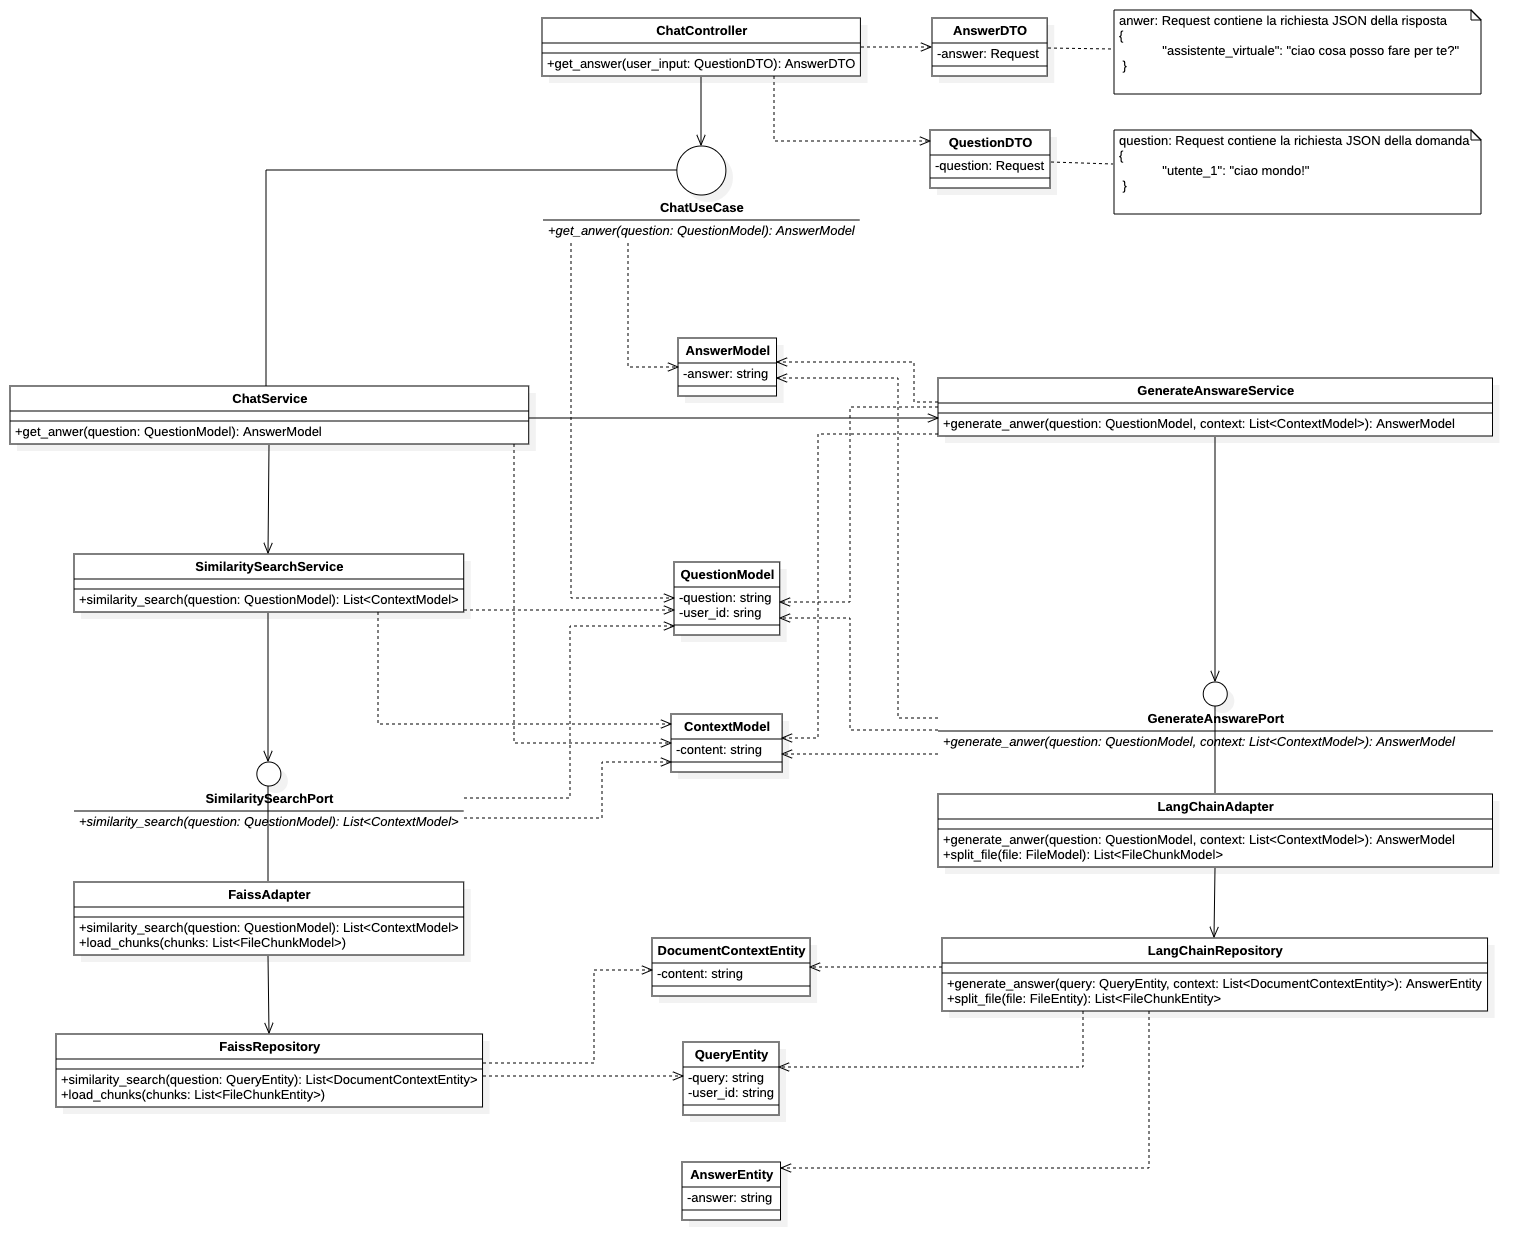
\includegraphics[width=\linewidth, height=0.8\textheight, keepaspectratio]{./img/ChatController.png}
    \caption{Diagramma delle classi - Chat Controller}
    \label{fig:chat_controller}
\end{figure}



\subsubsection{Add File Controller}
\begin{figure}[H]
    \centering
    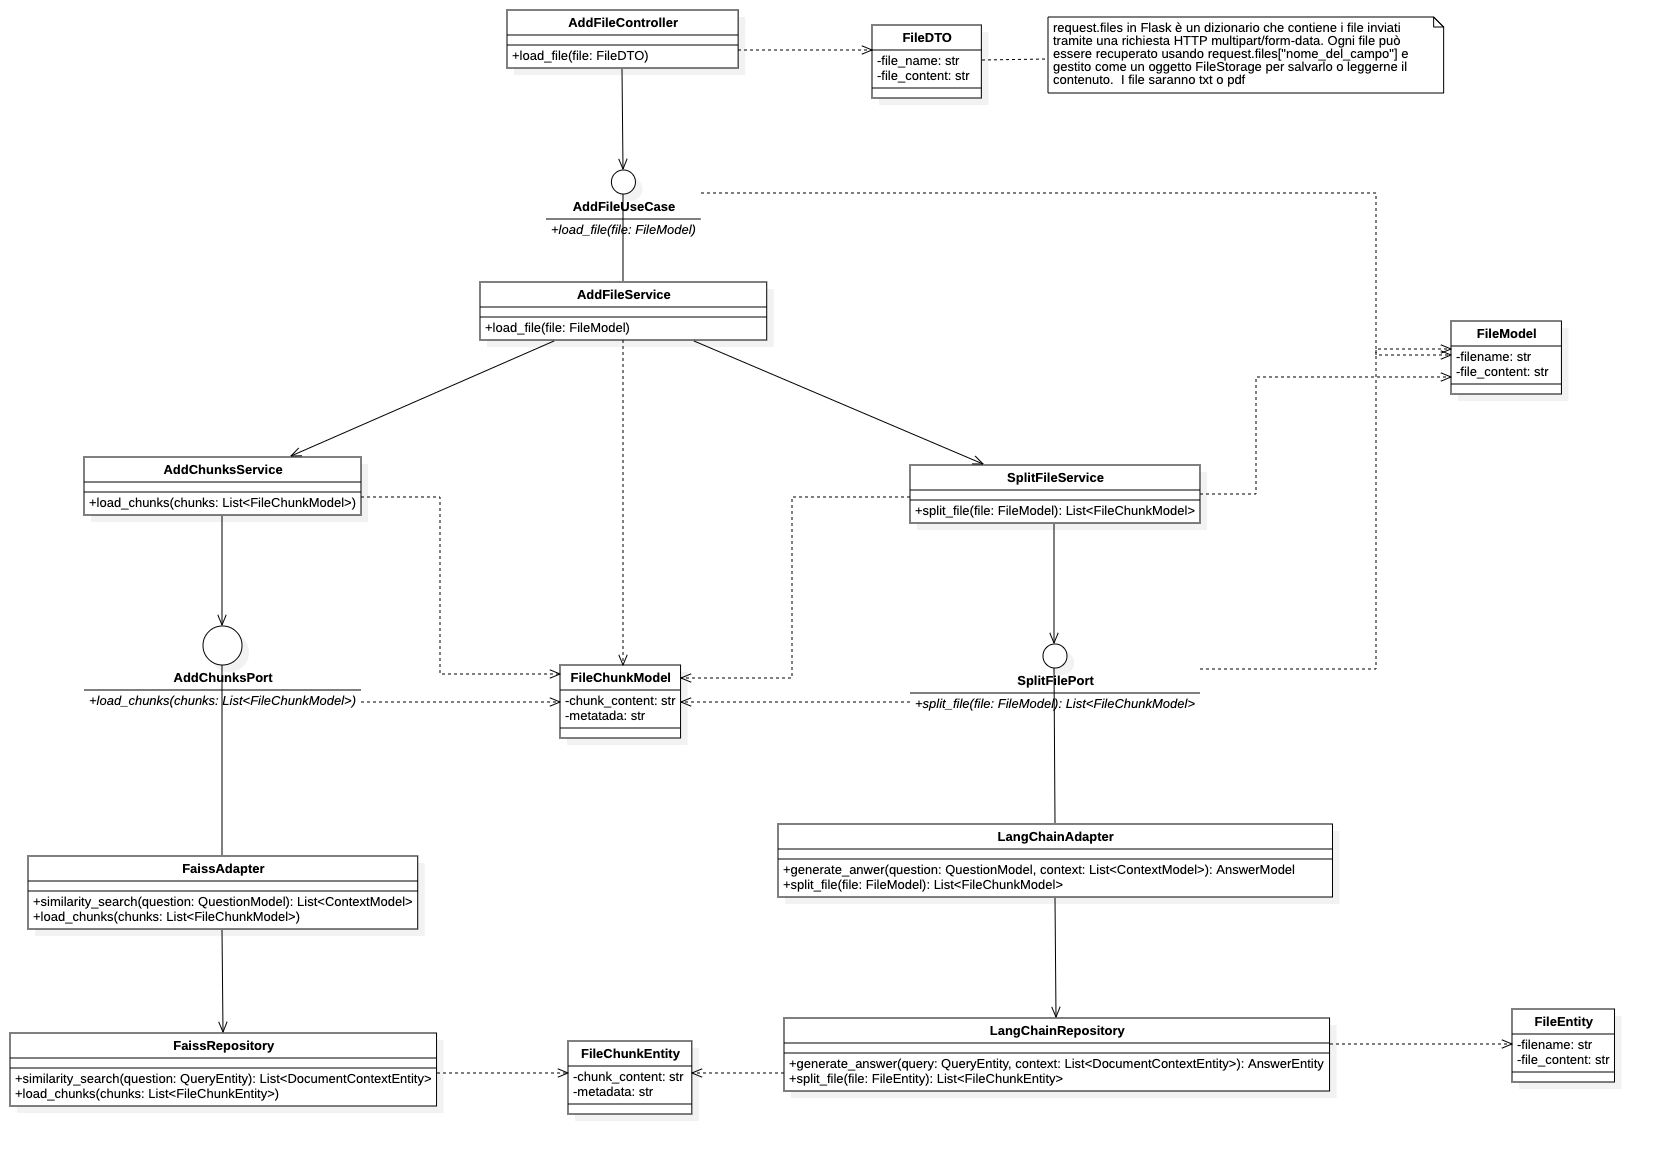
\includegraphics[width=\linewidth, height=0.8\textheight, keepaspectratio]{./img/AddFileController.png}
    \caption{Diagramma delle classi - Add File Controller}
    \label{fig:add_file_controller}
\end{figure}



\subsubsection{Conversation}
\begin{figure}[H]
    \centering
    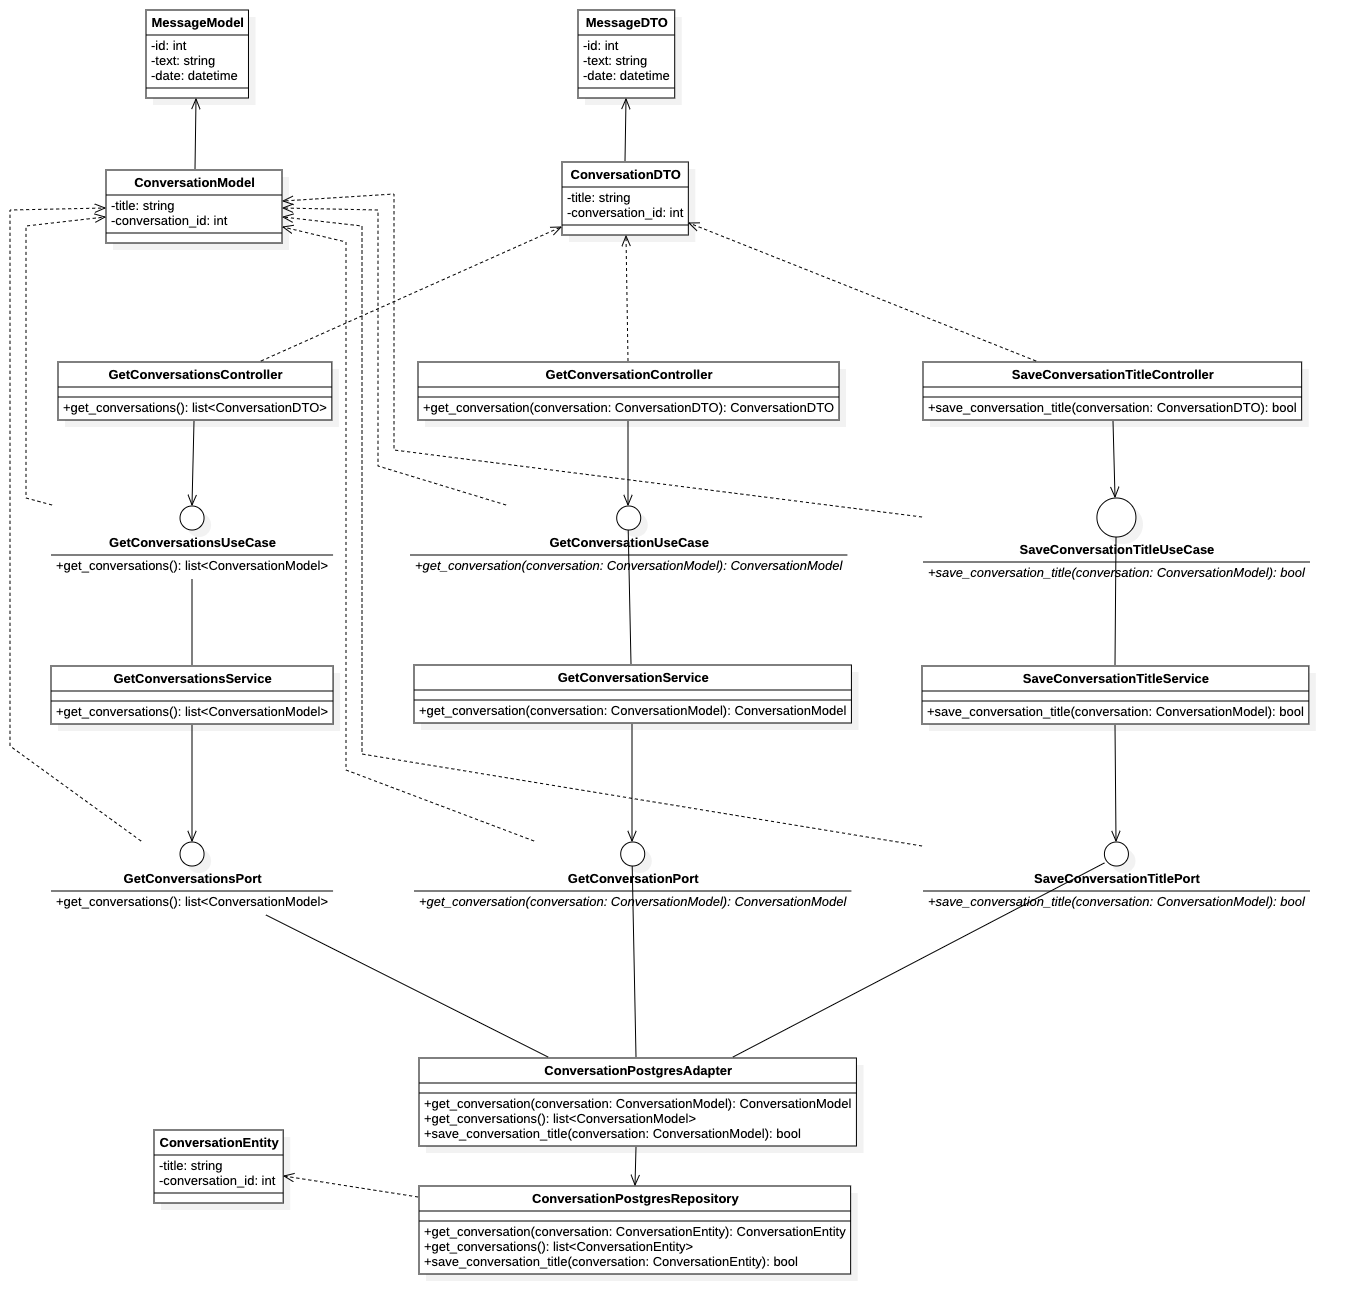
\includegraphics[width=\linewidth, height=0.8\textheight, keepaspectratio]{./img/Conversation.png}
    \caption{Diagramma delle classi - Conversation}
    \label{fig:conversation}
\end{figure}


\subsubsection{Message}
\begin{figure}[H]
    \centering
    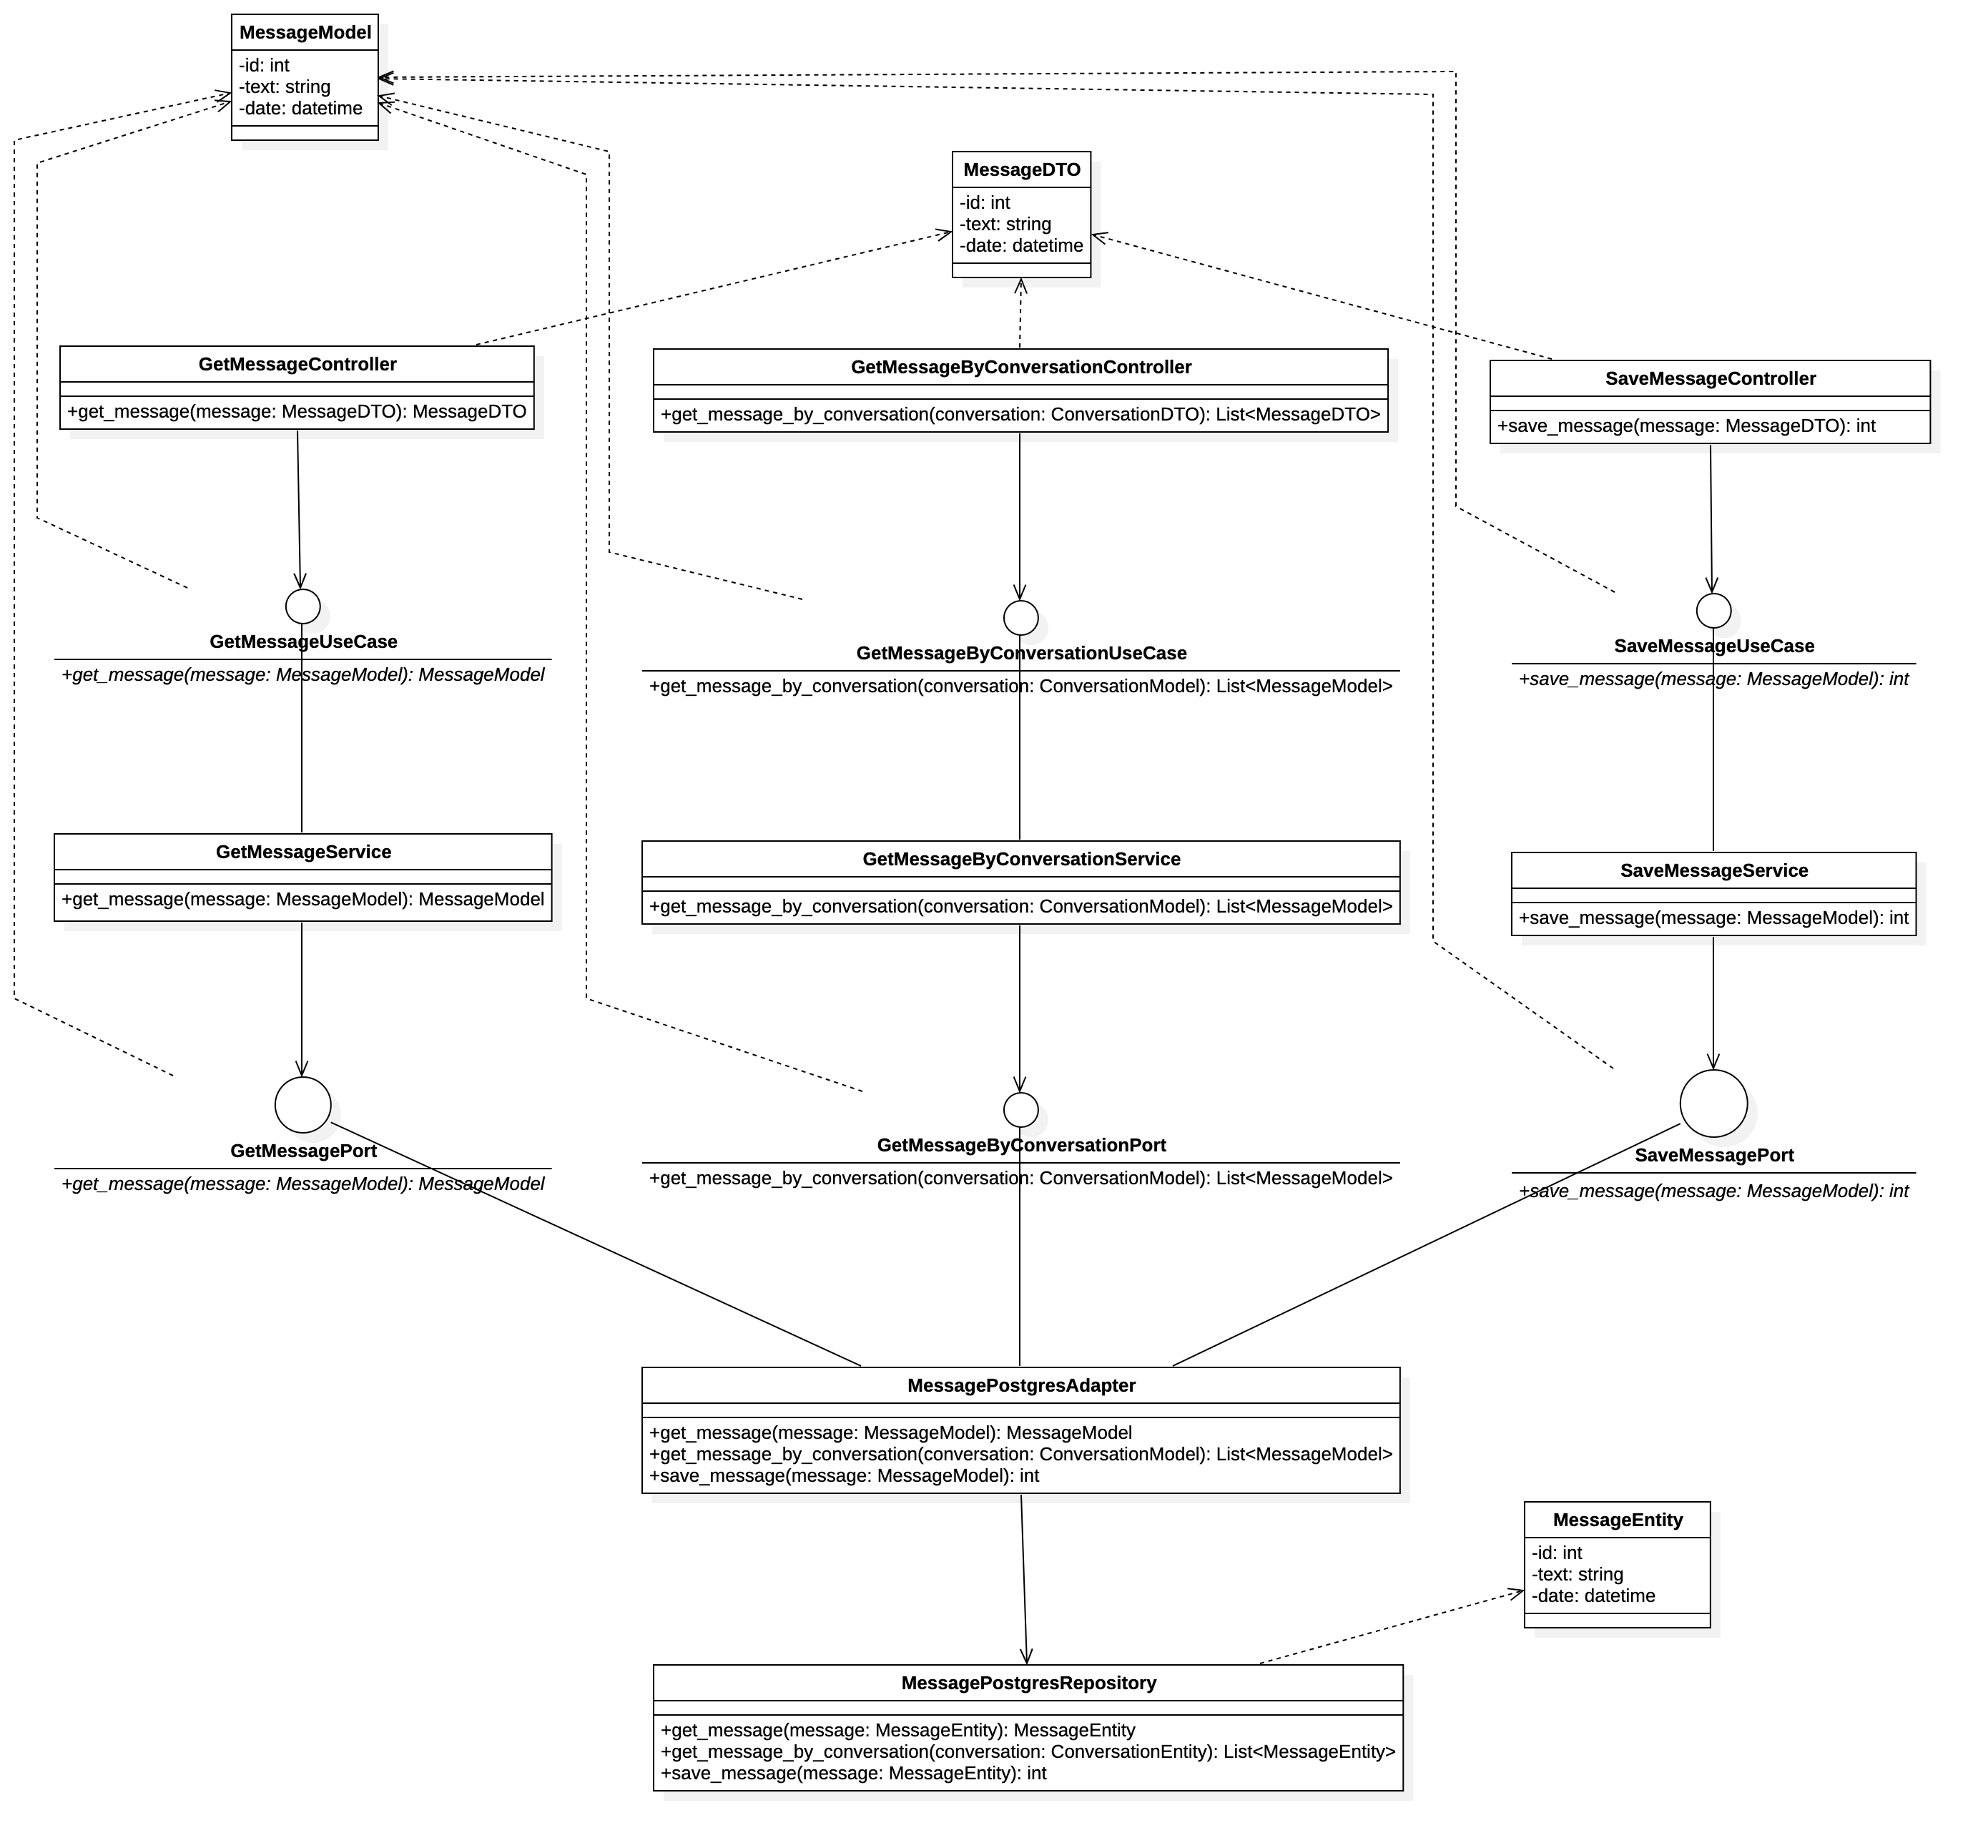
\includegraphics[width=\linewidth, height=0.8\textheight, keepaspectratio]{./img/Message.png}
    \caption{Diagramma delle classi - Message}
    \label{fig:message}
\end{figure}

\subsubsection{User}
\begin{figure}[H]
    \centering
    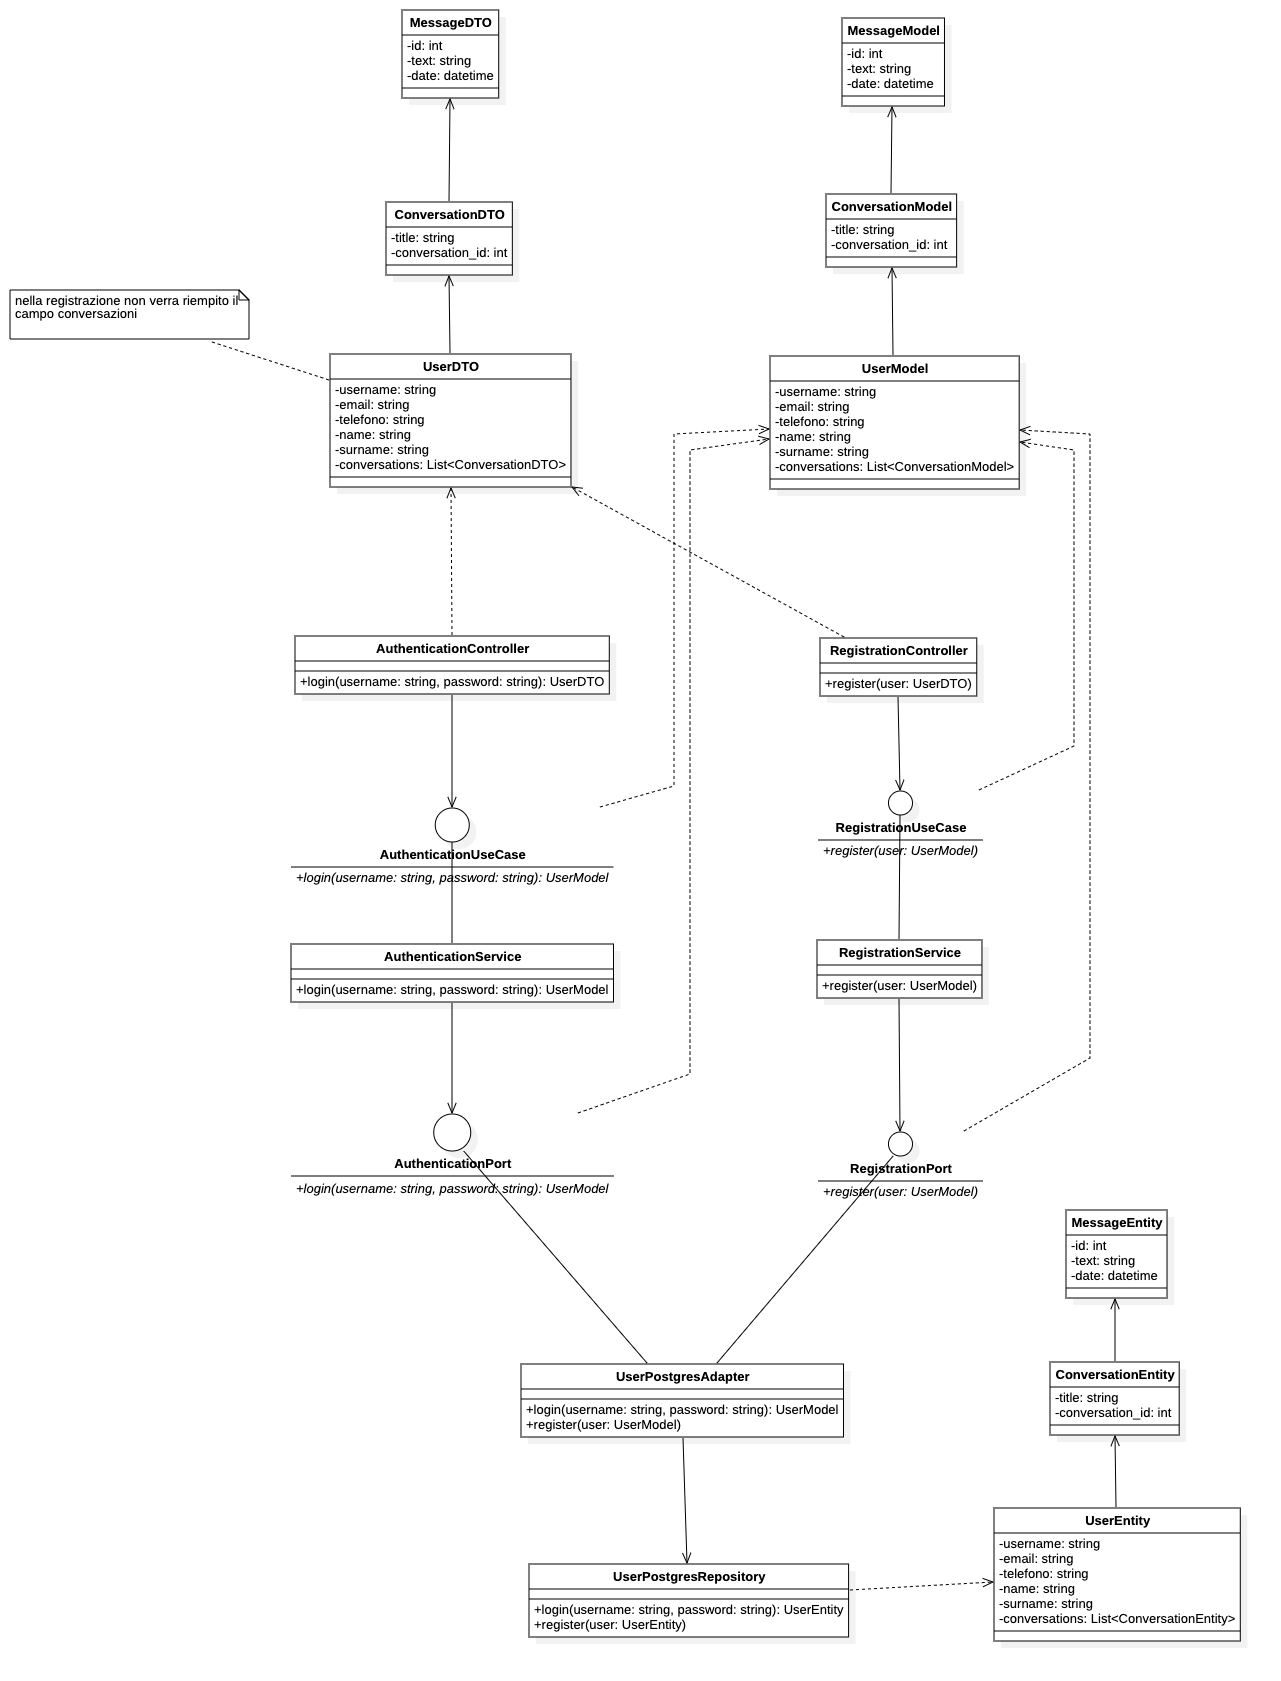
\includegraphics[width=\linewidth, height=0.8\textheight, keepaspectratio]{./img/User.png}
    \caption{Diagramma delle classi - User}
    \label{fig:user}
\end{figure}


\subsubsection{Support Message}
\begin{figure}[H]
    \centering
    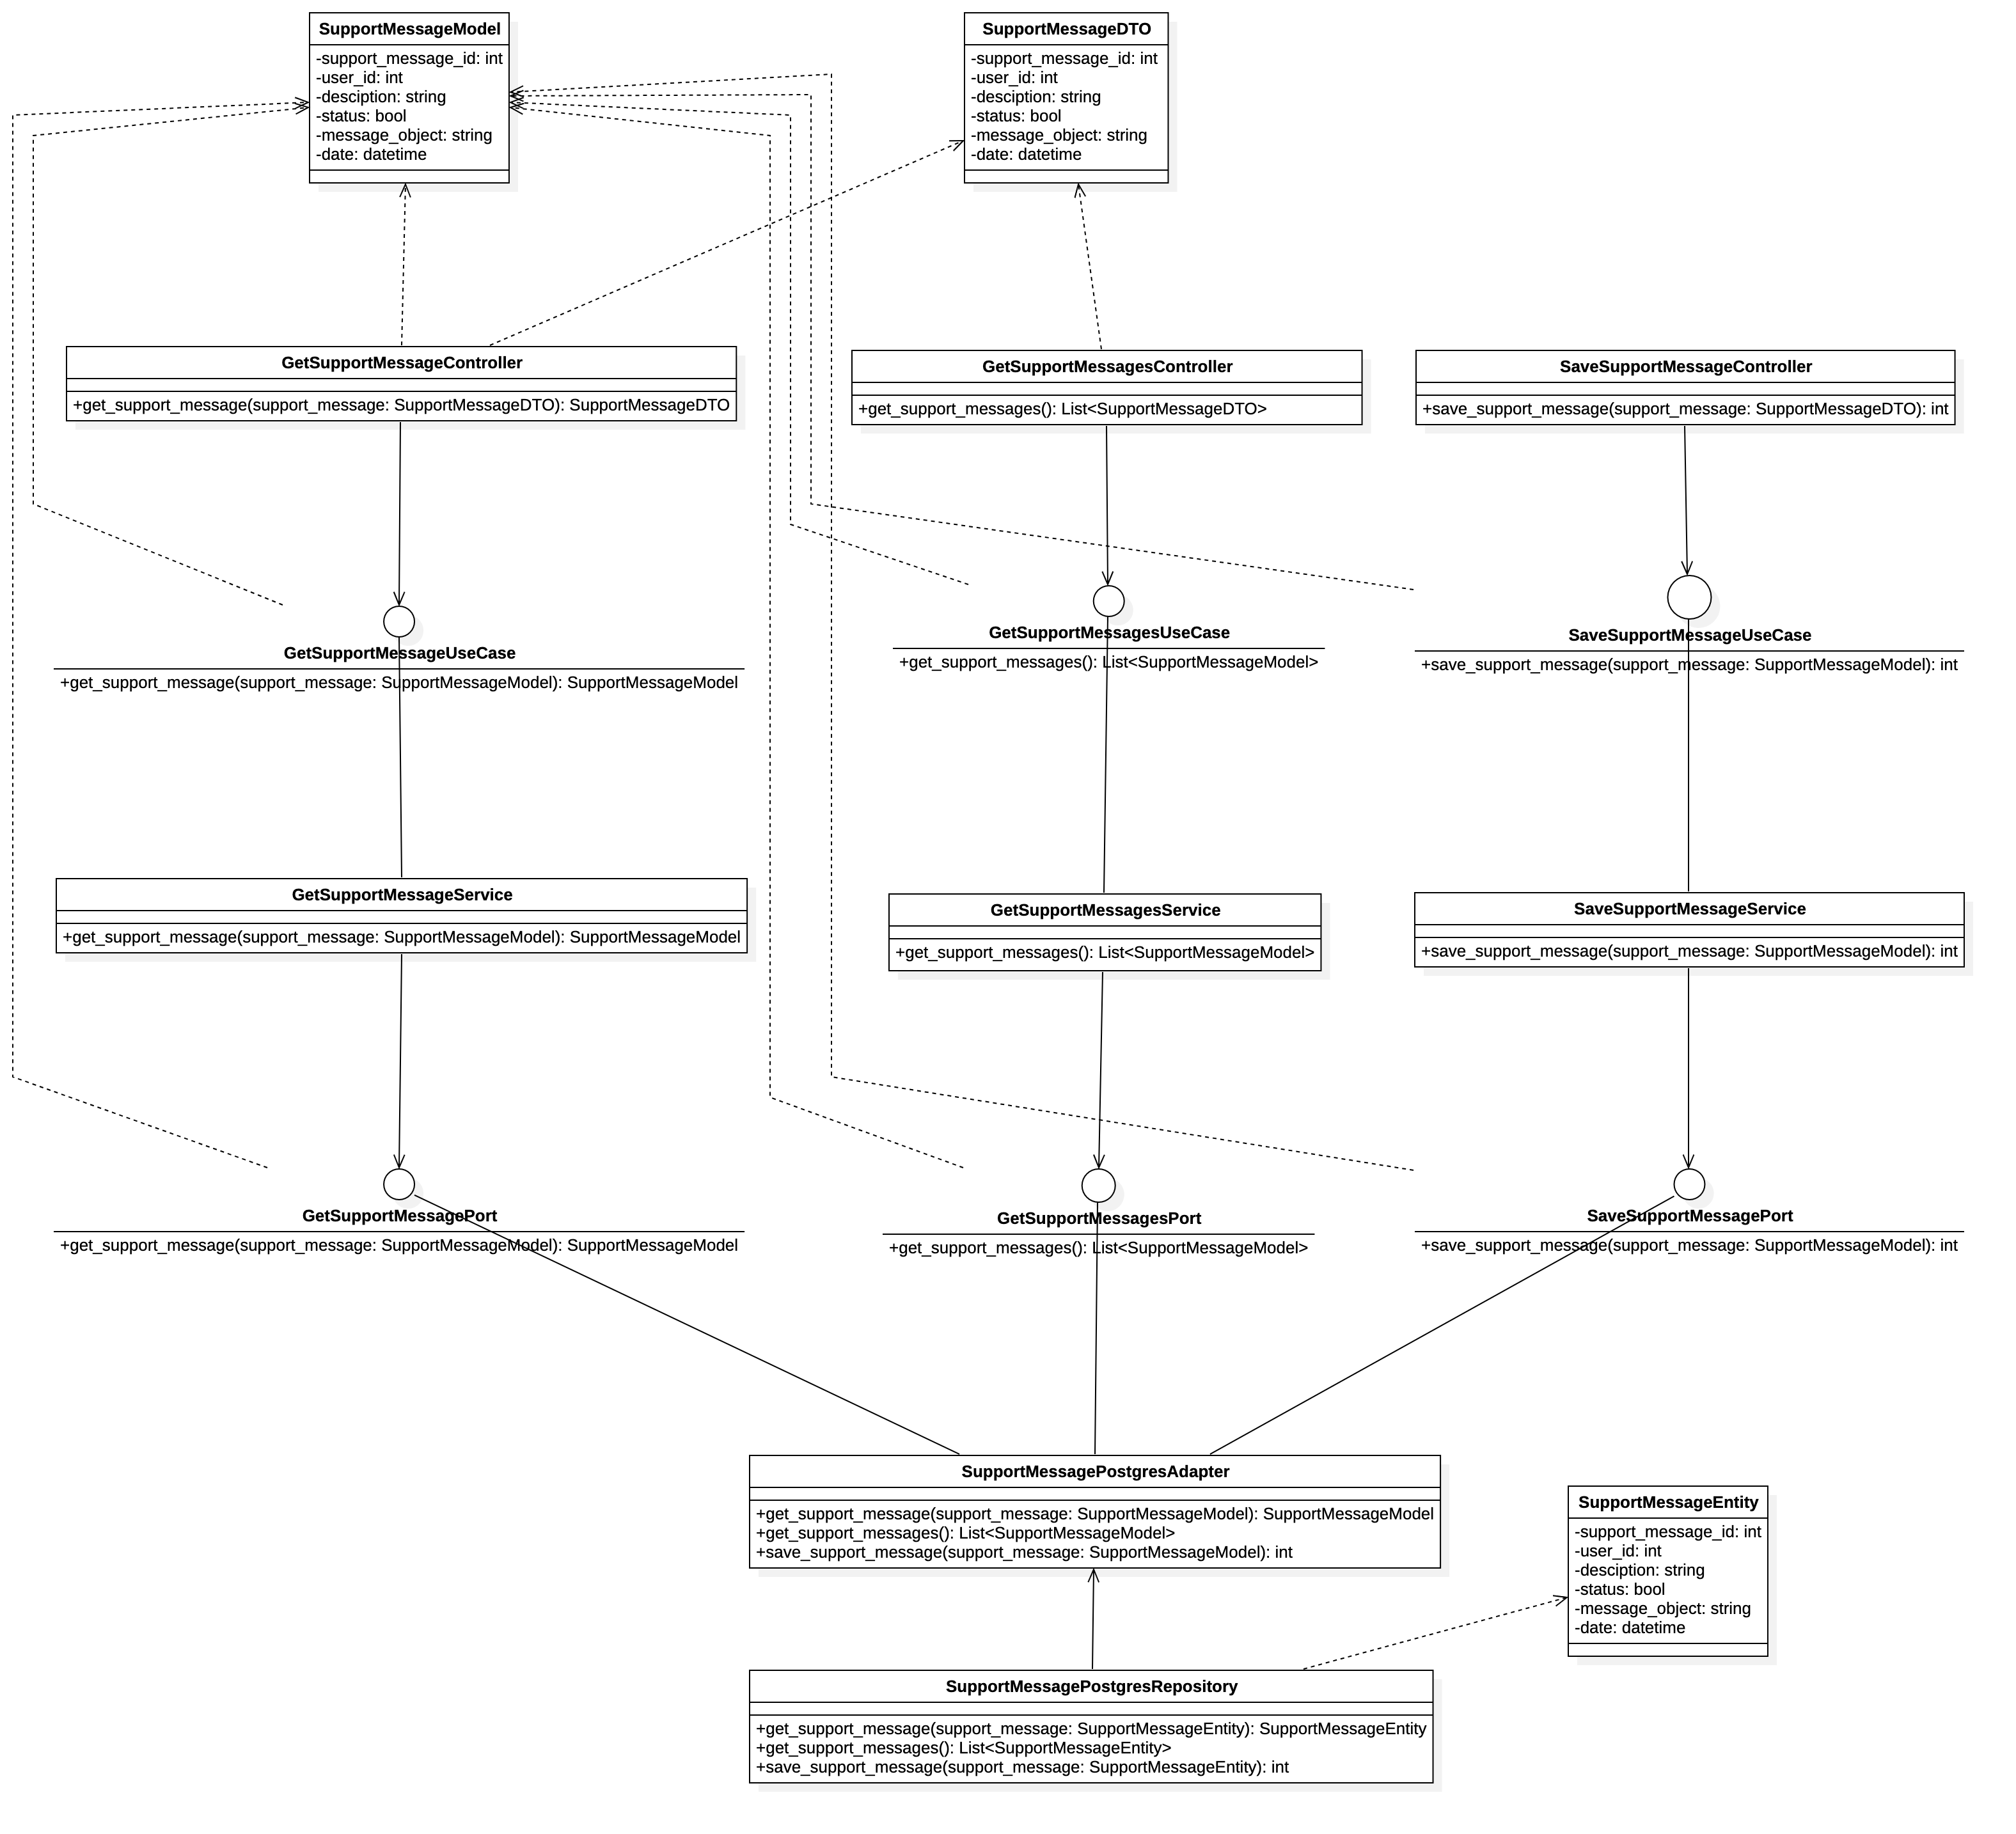
\includegraphics[width=\linewidth, height=0.8\textheight, keepaspectratio]{./img/SupportMessage.png}
    \caption{Diagramma delle classi - Support Message}
    \label{fig:support_message}
\end{figure}



\subsubsection{Template}
\begin{figure}[H]
    \centering
    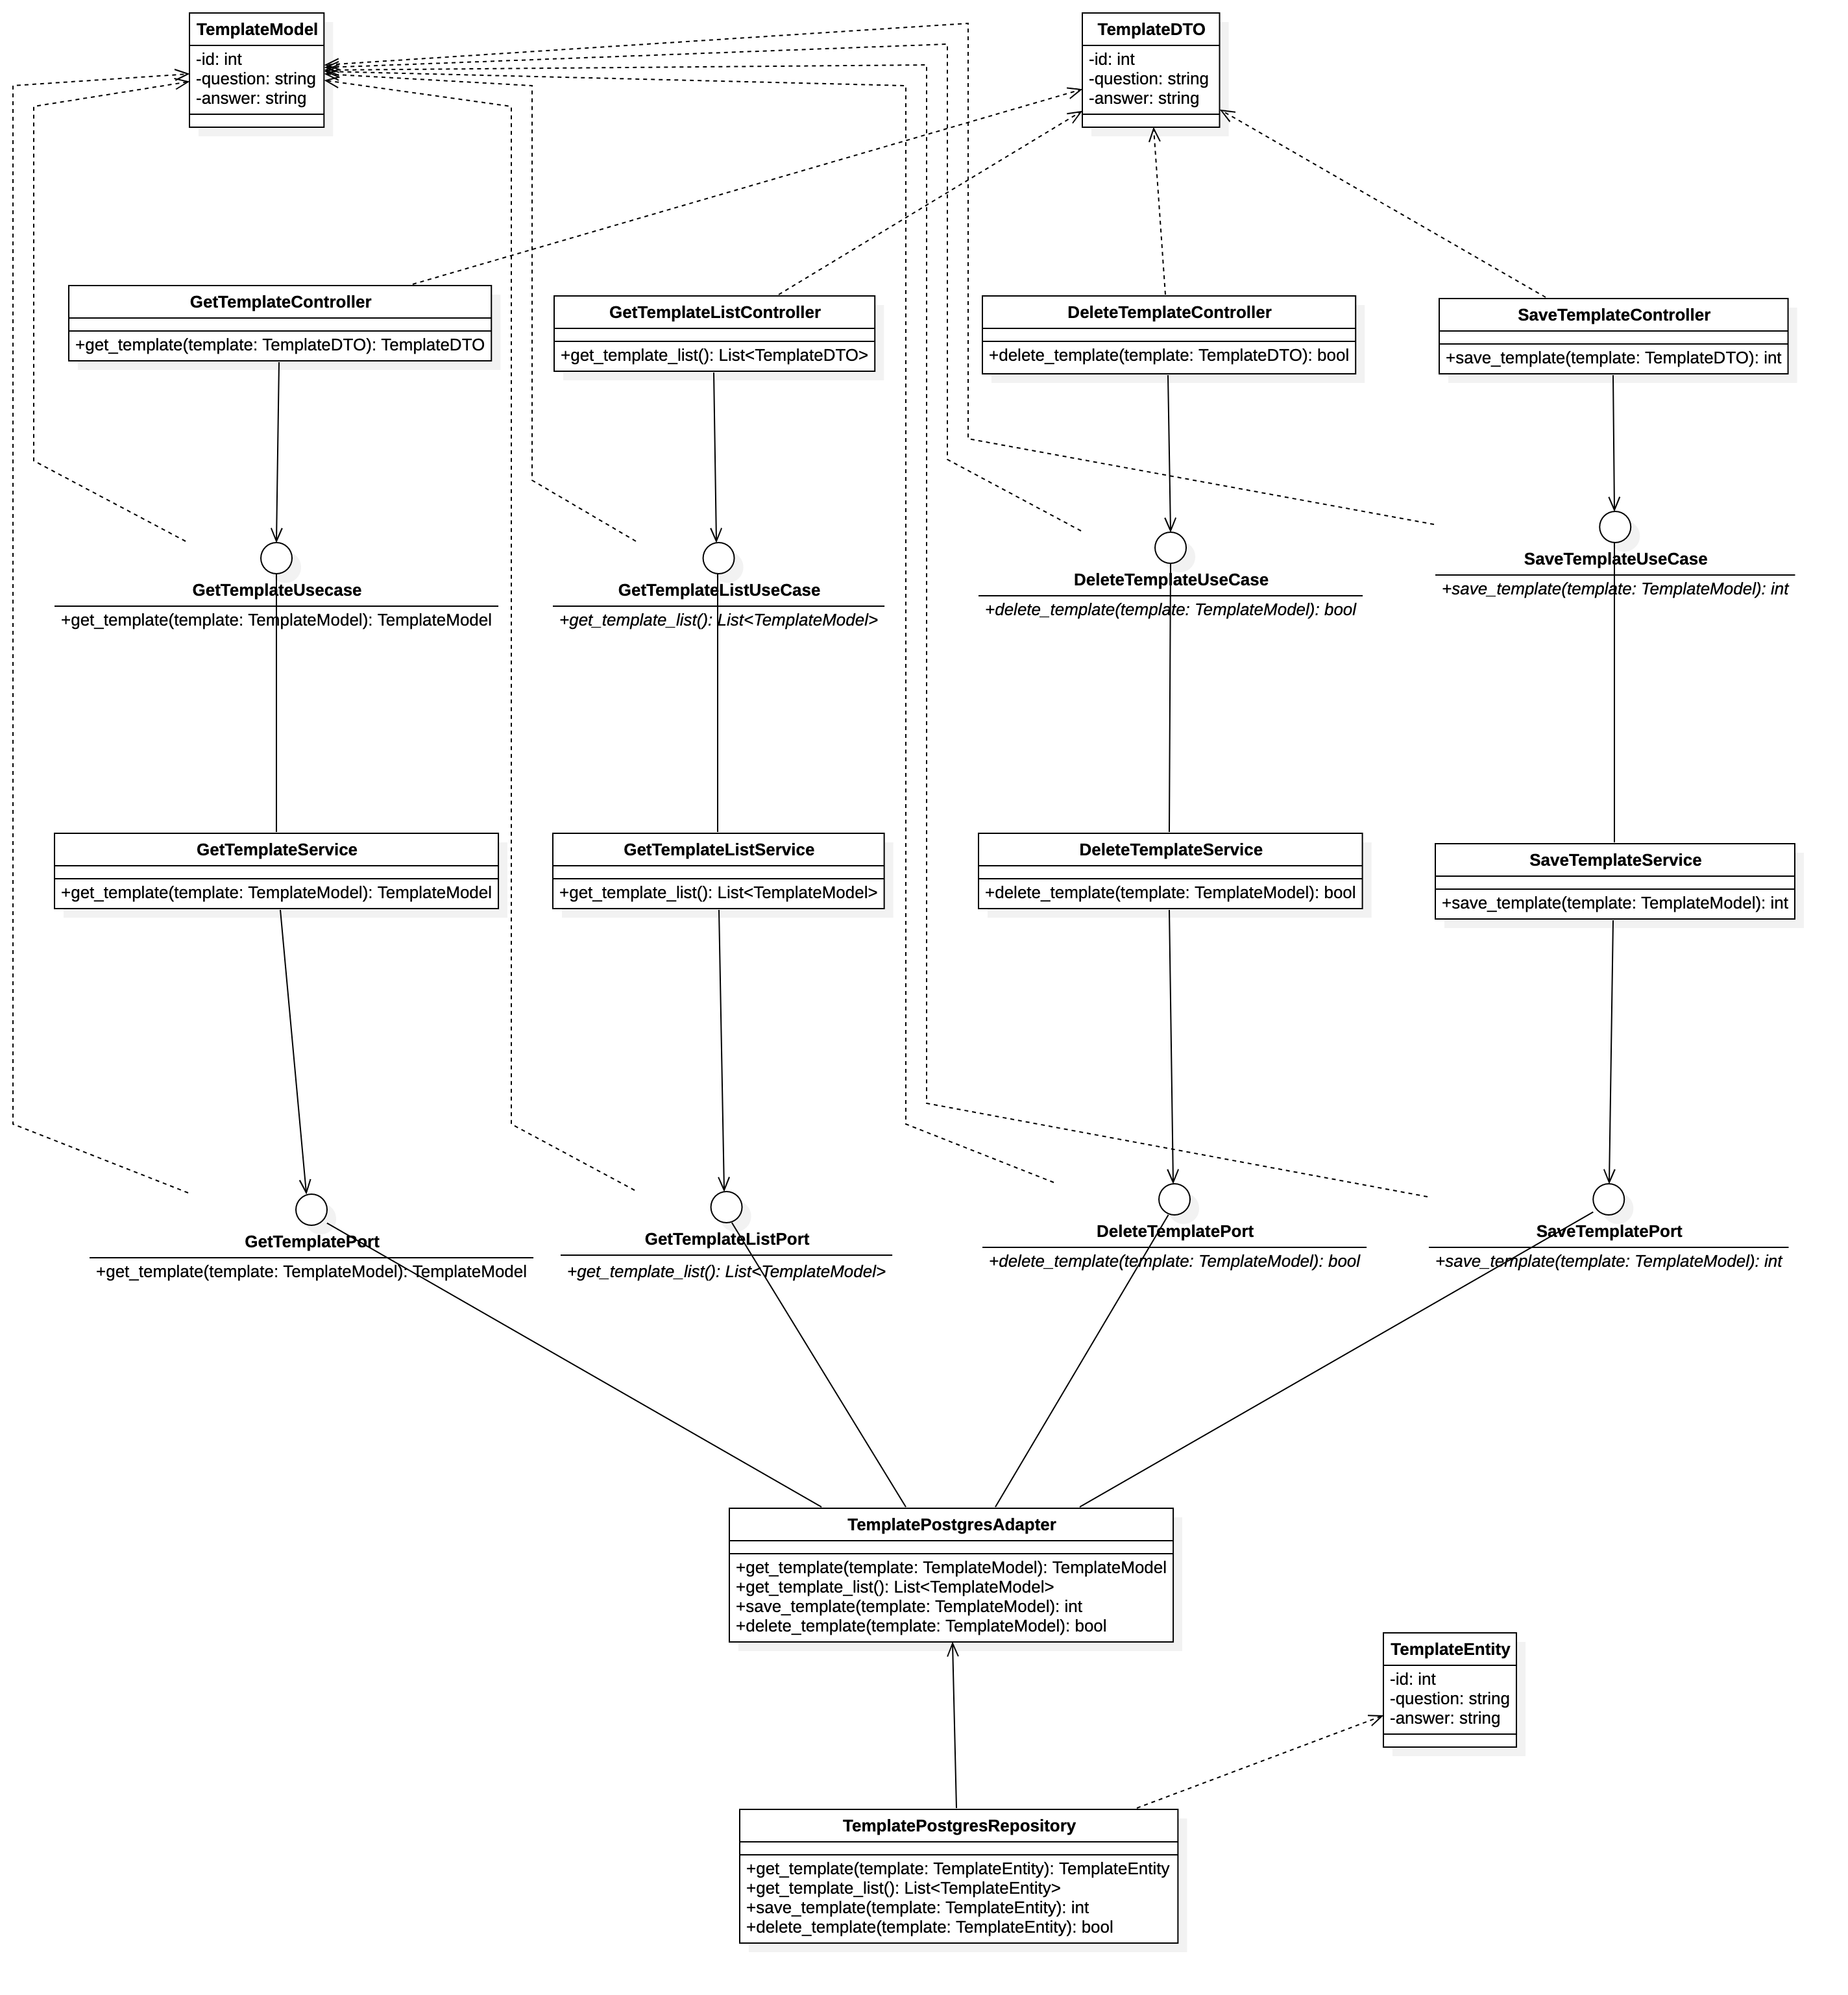
\includegraphics[width=\linewidth, height=0.8\textheight, keepaspectratio]{./img/Template.png}
    \caption{Diagramma delle classi - Template}
    \label{fig:template}
\end{figure}



%%%%%%%%%%%%%%%%%%%%%%%%%%%%%%%%%%%%%%%%%%%%%%%%%%%%%%%%%%%%%%%%%%%%%%%%%%%%%%%%%%
\subsection{Tecnologie}
%%%%%%%%%%%%%%%%%%%%%%%%%%%%%%%%%%%%%%%%%%%%%%%%%%%%%%%%%%%%%%%%%%%%%%%%%%%%%%%%%%
\subsubsection{OpenAI API}
%%%%%%%%%%%%%%%%%%%%%%%%%%%%%%%%%%%%%%%%%%%%%%%%%%%%%%%%%%%%%%%%%%%%%%%%%%%%%%%%%%

